\documentclass[tikz,border=2pt]{standalone}
\usepackage{amsmath,amssymb}
\usepackage{tikz}
\usetikzlibrary{arrows.meta}

\begin{document}
% For A = [[2,1],[1,2]] the eigenvectors (1,1) and (1,-1) are only stretched (by 3 and 1),
% while a generic vector is also turned.
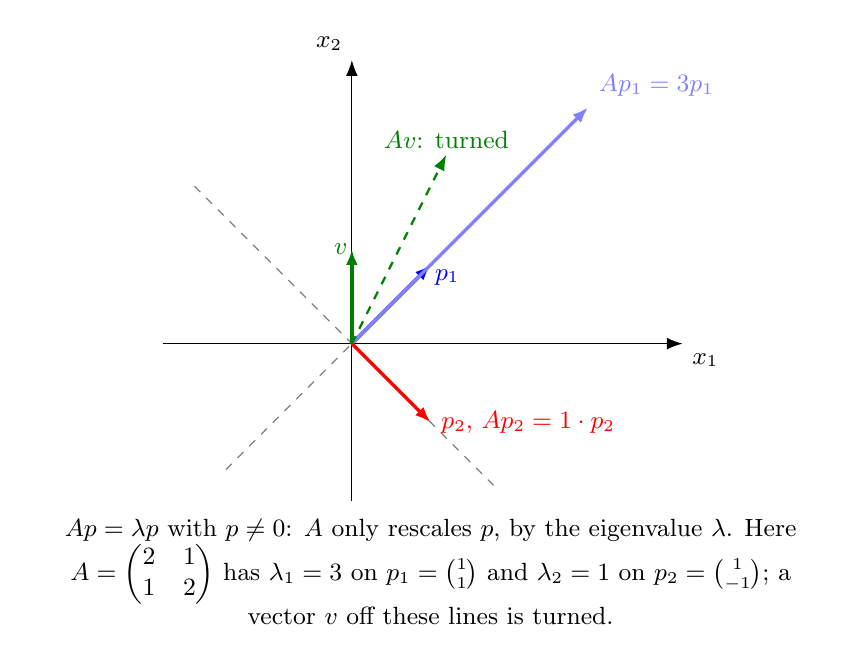
\begin{tikzpicture}[every node/.style={font=\small}, >={Latex[length=2mm]}]
	\draw[->] (-2.4,0) -- (4.2,0) node[below right] {$x_1$};
	\draw[->] (0,-2.0) -- (0,3.6) node[above left] {$x_2$};
	\draw[gray, dashed] (-1.6,-1.6) -- (3.0,3.0);
	\draw[gray, dashed] (-2.0,2.0) -- (1.8,-1.8);
	\draw[->, blue, very thick] (0,0) -- (1,1) node[below right, inner sep=1pt] {$p_1$};
	\draw[->, blue!50, very thick] (0,0) -- (3,3) node[above right] {$Ap_1=3p_1$};
	\draw[->, red, very thick] (0,0) -- (1,-1) node[right] {$p_2$, $Ap_2=1\cdot p_2$};
	\draw[->, green!50!black, very thick] (0,0) -- (0,1.2) node[left, inner sep=1pt] {$v$};
	\draw[->, green!50!black, thick, dashed] (0,0) -- (1.2,2.4) node[above, inner sep=2pt] {$Av$: turned};
	\node[anchor=north, align=flush center, text width=10cm] at (1,-2.1) {$Ap=\lambda p$ with $p\neq0$: $A$ only rescales $p$, by the eigenvalue $\lambda$. Here $A=\begin{pmatrix}2&1\\1&2\end{pmatrix}$ has $\lambda_1=3$ on $p_1=\binom11$ and $\lambda_2=1$ on $p_2=\binom1{-1}$; a vector $v$ off these lines is turned.};
\end{tikzpicture}
\end{document}
